% TITLE: Integrated in Knowledge, Unresolved in Organisations? A Preregistered Test for Structural Holes Between AI and Decision-Making

\section{Introduction}
\label{sec:intro}

Management and information-systems research increasingly treats artificial intelligence (AI) as a question of organisational decision-making. This work examines decision structures that combine human and AI decision-makers \citep{shrestha2019organizational}, the interdependence of automating and augmenting managerial tasks \citep{raisch2021artificial}, the complementary roles of humans and AI in organisational decisions \citep{jarrahi2018artificial}, and the distinctive management challenges raised by the autonomy, learning and inscrutability of AI \citep{berente2021managing}. Alongside this work, a common explanation for the distance between what AI can do and how it is used in managerial decisions is structural. AI and decision-making, the argument runs, form two weakly connected communities. In network terms, a structural hole separates them \citep{burt1992structural}, and actors who span it would gain information and control benefits \citep{burt2004structural}, in the way that weak ties carry information across otherwise separate groups \citep{granovetter1973strength}.

The premise has practical appeal. If such a hole exists, research can locate it and design bridges across it. The project reported here began with exactly this premise and used it to motivate a multi-level programming (MLP) model of how organisations allocate resources, govern AI and configure human--AI decisions. Before building further on the premise, this paper tests it.

A test requires data that can carry Burt's construct, and this is less straightforward than it appears. Structural holes are defined on the ego networks of actors linked by real relations of information or resource exchange. The standard measure, network constraint, is driven largely by degree and dyadic ties \citep{everett2020unpacking}, and recent work reads it as operationalising mainly dyadic constructs; this is a reinterpretation of structural-hole findings, not a refutation of the theory \citep{johnson2026reassessing}. Structural-hole measures also suit particular data types and cannot be substituted arbitrarily \citep{saglietto2020research}. Much of the evidence that could be offered for an AI--decision ``gap'', however, consists of co-occurrence: functions mentioned together in papers, or organisations that share projects. Co-occurrence records affiliation, not flow. In a strict two-mode graph the indirect term of constraint vanishes, and one-mode projections manufacture closure (Section~\ref{sec:theory_cooccurrence}). A valid test needs directed dyadic flows between actors that carry group labels. Patent citations, long used as evidence of knowledge flows \citep{jaffe1993geographic}, provide such relations.

We address three research questions. \textbf{RQ1:} Is there a structural hole between AI and decision-making as knowledge domains? \textbf{RQ2:} If not at the domain level, is there one at the organisational (firm) level, beyond what firms' technology portfolios mechanically imply? \textbf{RQ3/RQ4:} Given these answers, where should the integration problem be modelled, and how?

The evidence comes from three data lines (Figure~\ref{fig:research_design}). The first is the literature (Study~1): a corpus of 2,118 source documents whose evidence sentences were coded into 10 AI and 12 decision function families, together with network lines (V6--V11.1) that searched citation, co-author and higher-order networks for Burt brokers. The second is a screen of six public relational sources for flow validity. The third is a population of US utility patents (Study~2), in which AI is CPC G06N and decision-making (DEC) is CPC G06Q10/04 plus G06Q10/06. Study~2 comprises four preregistered analyses, each frozen in a public commit: an aggregate domain test, a test battery on a CPC cell matrix, a full replication suite and a portfolio-preserving firm null \citep{nosek2018preregistration}. The patent analyses at the domain, cell and firm levels share one source and are therefore not independent of one another. Study~3, set in one or more manufacturing firms, is preregistered as a plan and reports no results.

The findings are negative at the level of knowledge flows. AI and decision patents cite each other at a symmetric observed-to-expected intensity of 3.05 (95\% CI 2.94--3.17), higher than 97.8\% of comparable AI pairings and 92.2\% of comparable decision pairings. Both preregistered relative criteria for a hole fail, and the verdict, HOLE\_NOT\_SUPPORTED, is unchanged in all six sensitivity specifications (0/6 disagree). The over-connection declines over citing years (WLS slope $-0.097$ per year, 95\% CI $-0.130$ to $-0.065$) but carries the preregistered label PERSISTENT. Within the CPC matrix, cell-level depletions are small, and 0 depleted cells replicate in both time halves. At the firm level, specialist AI and decision firms are separated (O/E 0.24), but a portfolio-preserving null reproduces 85\% (primary stratification) and 91\% (technology-mix stratification) of that separation. Mixed-portfolio firms are more constrained than the null implies (median constraint 0.358 against null medians of 0.104 and 0.116), so they show no brokerage advantage; the preregistered verdict is PARTIAL. In the literature, the direction of 16 depleted function pairs is robust, but their significance does not survive realistic misclassification, given human inter-coder agreement of $\kappa$ = 0.05 (AI) and 0.14 (decision). The network lines, whose figures are HISTORICAL or USER\_REPORTED, confirmed 0 brokers, and none of the six public sources passed the flow-validity gates.

These results move the explanatory burden. If firms struggle to integrate AI into decisions, the binding constraints more plausibly lie inside organisations, in resource allocation, decision rights and governance, and human--AI configuration, where economic action is embedded in concrete relations \citep{granovetter1985economic}. We state this as a hypothesis. It is not a finding of Studies~1 and~2, which contain no organisation-internal data.

The paper makes four contributions. First, it reports a preregistered negative result: the knowledge-flow evidence does not support a structural hole between AI and decision-making as technology domains, which are instead over-connected. Second, it offers a measurement lesson for research on ``gaps'': co-occurrence and affiliation data cannot carry Burt's construct, and we document four specific failure modes (projection cliques, bipartite degeneration of constraint, same-term self-pairing and model-inferred labels). Third, it contributes two null models: M06-P, which replaces a document-preserving swap null that is degenerate on block-structured documents, and a portfolio-preserving firm null that separates brokerage from portfolio composition. Fourth, it reframes the integration problem as an organisational one, gives a formal tri-level programming model whose illustration uses simulated parameters only, and preregisters an enterprise study to calibrate it.

Section~\ref{sec:theory} develops the theoretical background and the measurement argument. Section~\ref{sec:design} sets out the research design, the preregistration log and the claim boundaries. Sections~\ref{sec:study1} and~\ref{sec:study2} report Studies~1 and~2. Section~\ref{sec:discussion} integrates the evidence, Section~\ref{sec:mlp} presents the MLP agenda and the plan for Study~3, Section~\ref{sec:limitations} discusses limitations and Section~\ref{sec:conclusion} concludes. Appendices~\ref{app:prereg}--\ref{app:mlp} contain the preregistration log, sensitivity tables and model details.

\section{Theoretical Background}
\label{sec:theory}

\subsection{Structural holes and their measurement}
\label{sec:theory_holes}

A structural hole is a separation between non-redundant contacts in an ego network. An actor whose contacts are not connected to one another receives non-redundant information and can play contacts off against each other; these are the information and control benefits of brokerage \citep{burt1992structural}. Managers who span structural holes have been argued to have better ideas, and brokerage in this sense presupposes real ties and observable outcomes \citep{burt2004structural}. The argument draws on the older observation that weak ties carry information across groups, whereas strong ties tend to overlap within communities \citep{granovetter1973strength}.

Burt's measure of the absence of such opportunities is network constraint:
\begin{equation}
c_i \;=\; \sum_{j \in N(i)} \Bigl( p_{ij} + \sum_{q \neq i,j} p_{iq}\, p_{qj} \Bigr)^{2},
\label{eq:constraint}
\end{equation}
where $N(i)$ is the set of $i$'s contacts and $p_{ij}$ is the proportional strength of $i$'s tie to $j$, that is, the weight of that tie as a share of all of $i$'s tie weights \citep{burt1992structural}. The direct term $p_{ij}$ records how much of $i$'s network is invested in $j$. The indirect term $\sum_{q} p_{iq} p_{qj}$ records how much of that investment is reached again through third parties $q$ who are themselves tied to $j$. Constraint is high when $i$'s ties are concentrated on few contacts and when those contacts are interconnected. Low constraint is read as access to structural holes.

Three lines of critique bear on how the measure can be used. First, constraint is driven by degree and dyadic ties; it is not a simple 0--1 index of exclusive brokerage \citep{everett2020unpacking}. Second, constraint operationalises mainly dyadic constructs (alternatives, partner diversity and concentration) rather than broader network structure. This calls for reinterpreting structural-hole findings; it does not refute the theory \citep{johnson2026reassessing}. Third, different structural-hole measures suit different data types and cannot be substituted for one another arbitrarily \citep{saglietto2020research}. Betweenness centrality, the share of shortest paths between other pairs that pass through a node \citep{freeman1977set}, is a common screen for intermediaries, but a high betweenness score alone does not establish Burt brokerage.

A more demanding definition of brokerage is relational and group-based. \citet{gould1989structures} define five brokerage roles on directed open two-paths, $s \rightarrow v \rightarrow t$ with no direct $s \rightarrow t$ tie, combined with the group membership of $s$, $v$ and $t$. \citet{zador2022weighted} extend these roles to a weighted and normalised measure that avoids the information lost through dichotomisation. Both formulations require that ties have a direction and that actors carry group labels.

We draw one requirement from this literature and apply it throughout. A valid test for a structural hole between two domains needs directed dyadic flow relations between actors that carry group labels. Measures computed on other kinds of data, such as constraint on affiliation graphs or betweenness on projected networks, may describe structure, but they do not test Burt's construct. Study~2 therefore uses directed applicant citations between examiner-labelled groups. It compares group-level intensities against a relative reference set and applies Burt constraint only to a firm-to-firm citation network, under a null model that preserves firms' portfolios (Section~\ref{sec:study2}).

\subsection{AI and decision-making as knowledge domains}
\label{sec:theory_domains}

Management and information-systems scholarship treats the meeting of AI and decision-making as a matter of organisational design: how decisions are structured across humans and AI \citep{shrestha2019organizational}, how automation and augmentation are balanced \citep{raisch2021artificial}, how humans and AI complement one another \citep{jarrahi2018artificial}, and how AI is to be managed \citep{berente2021managing}. The structural-hole premise makes a narrower claim about knowledge: that AI and decision-making form separate bodies of knowledge with few connections between them. We operationalise the two domains accordingly. In Study~1, a domain is a family of functions coded from evidence sentences in the literature: 10 AI families and 12 decision families, giving 120 cells. In Study~2, a domain is a set of examiner-assigned Cooperative Patent Classification (CPC) labels. AI is G06N. DEC is G06Q10/04 (forecasting and optimisation) plus G06Q10/06 (resources, workflow, management and decision analysis).

Patent citations record the prior art on which an invention builds, and they have long been used as evidence of knowledge flows \citep{jaffe1993geographic}. A large share of citations, however, is added by examiners, which affects their use as a flow measure; inventor or applicant citations should be distinguished from examiner citations \citep{alcacer2006patent}. The primary specification of Study~2 therefore uses applicant citations only, and a preregistered sensitivity check uses all citation categories. The data are the PatentsView granted-patent tables, which provide patents, current CPC classifications, citations and disambiguated assignees \citep{uspto2026patentsview}.

The domain test must be relative. Citing is field-local, so the observed-to-expected ratio (OE) of citations between almost any two fields is usually below 1. An absolute criterion of ``OE below 1'' would therefore flag nearly every pair of fields as separated. Study~2 instead asks whether the AI--DEC pair is unusually weakly connected compared with similar pairs. Hypothesis H1a places OE(AI,DEC) in the lowest quartile of AI's and DEC's intensities with 179 comparable CPC main groups. Hypothesis H1b requires the ratio of OE(AI,DEC) to OE(AI, other business methods) to lie below 1, with its upper confidence bound also below 1. Formal definitions are given in Section~\ref{sec:study2}.

The same knowledge flows also run between organisations. Firms hold specialist AI portfolios, specialist decision portfolios or mixed portfolios, and the economic action that combines them is embedded in concrete relations between and within organisations \citep{granovetter1985economic}. RQ2 asks whether a separation exists at this level that firms' portfolios do not already explain.

\subsection{Why co-occurrence is not flow}
\label{sec:theory_cooccurrence}

Much of the material that could be offered as evidence of AI--decision ``gaps'', including the matrix of Study~1, is co-occurrence: an AI function and a decision function mentioned in the same paper, or two organisations participating in the same project. Such data are two-mode, or affiliation, data. They link actors to events, not actors to actors, and they record no direction of transfer.

Applying constraint to a strict bipartite graph has a formal consequence. Let $i$ belong to one mode. Every contact $j \in N(i)$ then belongs to the other mode, and so does every third party $q$ with $p_{iq} > 0$. Because $q$ and $j$ belong to the same mode, they cannot be tied, so $p_{qj} = 0$, and the indirect term in Eq.~\eqref{eq:constraint} is identically zero. Constraint reduces to $c_i = \sum_{j} p_{ij}^{2}$. If, in addition, all of $i$'s ties have equal weight, then $p_{ij} = 1/k_i$ for each of $i$'s $k_i$ contacts, and $c_i = 1/k_i$. Under this equal-weight condition, constraint carries no information beyond degree. The Gap Validity sidecar of Study~1 and check P9 of Study~2 both confirm the zero indirect term in their bipartite networks (Sections~\ref{sec:study1} and~\ref{sec:study2}).

Projection does not repair the problem. Co-authorship networks, for example, are built from article--author two-mode data projected to one mode \citep{newman2001scientific}, and we do not treat co-authorship as direct evidence of knowledge flow. One-mode projection creates artificial closure, which is why clustering must be redefined for two-mode data \citep{opsahl2013triadic}. Brokerage computed after projection is not brokerage on open two-paths in the sense of \citet{gould1989structures}, because projection closes the very two-paths on which those roles are defined; two-mode brokerage chains are one alternative \citep{jasny2015two}. Our own data illustrate the size of the distortion. In the CORDIS H2020 project data screened for this study, the co-membership projection of keyword-matched organisations has 1,049 nodes and 12,181 edges. It creates 102,660 within-project triads, whereas only 156 edges recur across $\geq 2$ projects.

Study~1 reveals two further failure modes, which Section~\ref{sec:study1} details. The first is same-term self-pairing: in the strongest enriched cell (prediction $\times$ prediction), 33\% of records pair the same term on both sides, so the ``co-occurrence'' partly reflects one word coded twice. The second is model-inferred labels with low human reliability. Agreement between two human coders on the function families was $\kappa$ = 0.05 (AI) and 0.14 (decision), where $\kappa$ is Cohen's chance-corrected agreement \citep{cohen1960coefficient}.

Burt's construct needs directed dyadic flows between labelled actors. Patent citations provide them: a citing patent draws on a cited patent, and both carry examiner-assigned classes. This motivates Study~2.

\section{Research Design and Preregistration}
\label{sec:design}

\subsection{Overview of the three studies}
\label{sec:design_overview}

Figure~\ref{fig:research_design} and Table~\ref{tab:front_overview} summarise the design. RQ1 is addressed by Study~1 (literature) and by the domain-level and cell-level analyses of Study~2 (patents). RQ2 is addressed by the firm-level analyses of Study~2. RQ3 and RQ4 are addressed by the MLP agenda in Section~\ref{sec:mlp} and by Study~3, a preregistered enterprise study that is a plan, not a source of results. The three data lines are (i) the literature (Study~1), (ii) six public relational sources screened for flow validity, and (iii) US patent citations at the domain, cell and firm levels (Study~2). Only line (iii) proved flow-valid, and its analyses at the three levels share one source.

\begin{figure}[t]
\centering
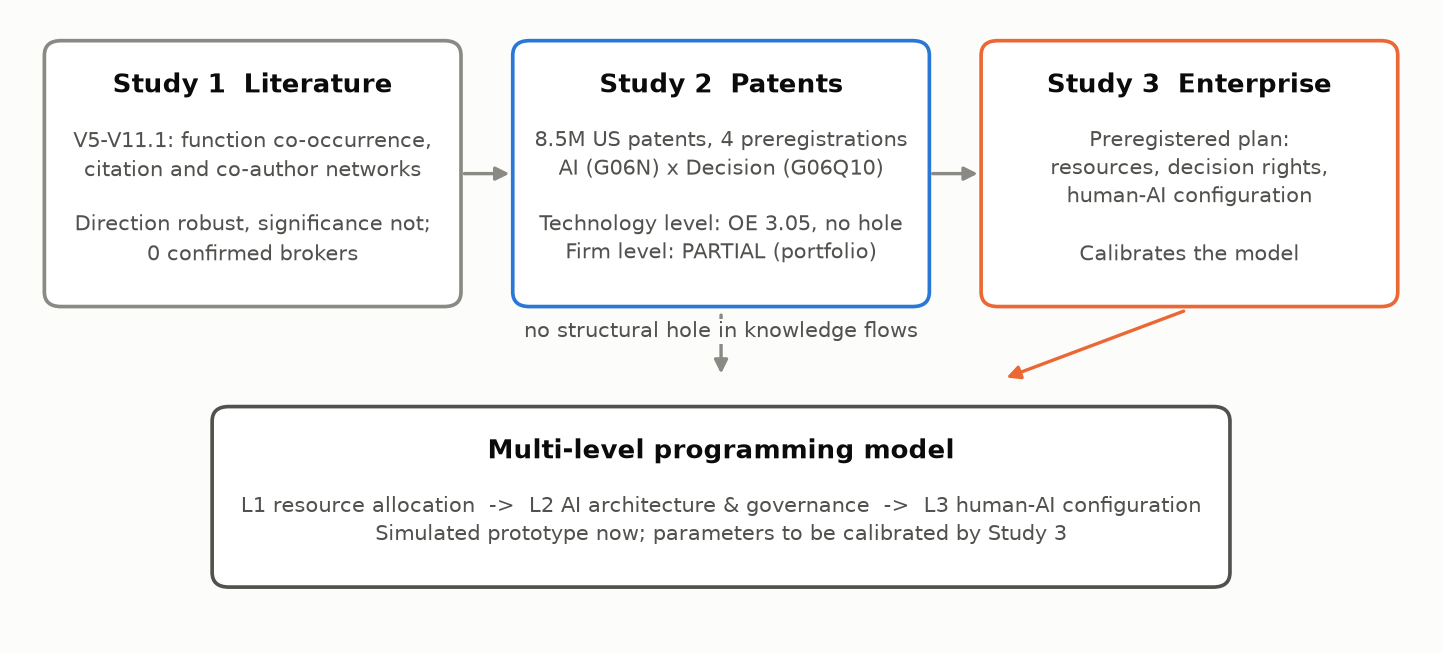
\includegraphics[width=\linewidth]{fig_research_design.png}
\caption{Research design. Study~1 (literature, V5--V11.1) and Study~2 (US patents; four preregistrations; AI = CPC G06N, Decision = CPC G06Q10/04 and G06Q10/06) address RQ1 and RQ2. Study~3 is a preregistered enterprise plan with no results yet; it is intended to calibrate the tri-level programming model (Level~1 resource allocation, Level~2 AI architecture and governance, Level~3 human--AI configuration), whose parameters are at present simulated. The rounded patent count in the figure corresponds to 8,512,829 utility patents; ``OE 3.05'' is the aggregate symmetric intensity; ``PARTIAL'' is the verdict of the portfolio-preserving firm null. The arrow label ``no structural hole in knowledge flows'' is shorthand: the evidence does not support a knowledge-flow structural hole (HOLE\_NOT\_SUPPORTED); it does not prove that none exists.}
\label{fig:research_design}
\end{figure}

\begin{table}[t]
\centering
\small
\caption{Overview of studies and data lines. Provenance grades are defined in Section~\ref{sec:design_prereg}.}
\label{tab:front_overview}
\begin{tabular}{@{}p{2.5cm}p{3.6cm}p{2.3cm}p{3.4cm}p{1.9cm}p{1.3cm}@{}}
\toprule
Study / line & Data & Relation type & Main tests & Grade & Status \\
\midrule
Study~1: functional matrix & 2,118 source documents; 2,180 document-level edges in a 10 $\times$ 12 matrix & Co-occurrence (two-mode) & Four null tests with BH-FDR; misclassification bound and simulation & DIRECT & Completed \\
Study~1: network lines V6--V11.1 & Citation, co-author and higher-order networks & Citation screens and projections & Search for Burt brokers; external review & HISTORICAL / USER\_REPORTED & Completed \\
External-data screen & Six public sources (CORDIS H2020, GLEIF, OpenAlex, OCDS, SEC, PyPSA) & Affiliation, ownership, physical topology & Independent-relation and validation gates & DIRECT & Completed \\
Study~2: patents & 8,512,829 US utility patents; AI = G06N, DEC = G06Q10/04 + G06Q10/06 & Directed applicant citations & Four preregistered plans: aggregate test, CPC matrix, replication suite, firm null & DIRECT & Completed \\
MLP prototype & 3 processes; regimes C/F/D; budgets 3/5/7 & None (simulated parameters) & Exact backward induction & SIMULATED & Illustration \\
Study~3: enterprise & Decision processes in one or more manufacturing firms & Planned enterprise data & Preregistered decision rules & -- & Plan \\
\bottomrule
\end{tabular}
\end{table}

\subsection{Selecting a flow-valid data source}
\label{sec:design_sources}

Before turning to patents, we screened six public relational sources against two gates, an independent-relation gate and a validation gate. CORDIS H2020 (35,389 projects; 179,063 organisation participations) yields co-membership, not flow. Under a degree-preserving bipartite swap null with 49 replicates, its 5 testable low-constraint candidates had $p$ = .41--.86 and BH $q \geq .80$ \citep{benjamini1995controlling}; 0 were significant. GLEIF Level-2 (663,449 relationship records, 481,247 active) records legal consolidation. OpenAlex returned 8 works, OCDS 0 verifiable buyer--supplier edges, and PyPSA (8,786 buses) describes a physical grid. SEC filings were not fetched because access requires a genuine contact User-Agent. No source passed both gates: co-membership, ownership and physical topology are not information flows. Appendix~\ref{app:sens} reports the full screen.

Patents meet the requirement of Section~\ref{sec:theory_holes}. Citations are directed flows \citep{jaffe1993geographic}, CPC classes are labels assigned by examiners rather than by the analyst, and the data cover the population of granted US patents rather than a sample.

\subsection{Preregistration log and provenance grades}
\label{sec:design_prereg}

Study~2 was preregistered in four plans, each frozen in a public commit of the project repository: the aggregate test (a8f3289), the V9 battery on the CPC matrix (a6266f7), the full replication suite (d641256) and the portfolio-preserving firm null (b59fc71), all in PR~\#5. The aggregate test was frozen before any patent data were downloaded. The three later plans were frozen before the analyses they govern were computed. Preregistration in this sense separates confirmatory from exploratory analysis by fixing the plan before outcomes are observed \citep{nosek2018preregistration}. Each plan fixed definitions, null models, decision rules, sensitivity checks and stop rules.

Deviations are recorded as dated amendments that leave the frozen text unchanged. Amendment A1 corrected the spelling of the CPC label for inventive codes before any citation result was computed; it did not change the design, groups, thresholds or decision rules. Amendment A2, a data note recorded after the run, documents that PatentsView labels non-examiner citations ``cited by other'' before 2013, so the applicant-only specification effectively covers citing years 2013--2025. Amendment B1 records that the preregistered document-preserving swap null accepted 0 of 21,843,600 swaps on patent data, which made the preregistered core uninformative by construction and led to the patent-adapted null M06-P (Section~\ref{sec:study2}). Appendix~\ref{app:prereg} gives the full log.

Before real data were analysed, the aggregate test was calibrated on synthetic networks. With no planted hole, the decision rule returned HOLE\_NOT\_SUPPORTED (ratio 0.99, 0.79--1.21). With a planted 30\% suppression (ratio 0.66, 0.52--0.83) and a planted 50\% suppression (ratio 0.47), it detected the hole. The test can therefore detect a hole of this size when one is present. Study~1's frozen V9 analysis used fixed seeds (20260918 for the stub Monte Carlo and 20260919 for the document-preserving swap), and its data-validity re-analysis is reported as post hoc.

Every number in the paper derives from a logged result file with one of three provenance grades. DIRECT numbers were recomputed or parsed from frozen files. HISTORICAL numbers were reported in earlier project logs whose raw files were not available for re-verification. USER\_REPORTED numbers were reported by the researcher from files held locally. We state the grade wherever it matters; the V6--V11.1 network results are HISTORICAL or USER\_REPORTED, and the MLP outputs are SIMULATED.

\subsection{Claim boundaries}
\label{sec:design_boundaries}

The following boundaries govern every claim in the paper:
\begin{enumerate}
\item[(i)] No confirmed structural hole is claimed at any level.
\item[(ii)] The 16 V9 depleted cells and the 5 patent cells depleted in both parts of the CPC matrix are not called research gaps.
\item[(iii)] No causal effects are claimed.
\item[(iv)] MLP outputs are simulated and reflect no real firm.
\item[(v)] ``The bottleneck is organisational'' is a hypothesis for Study~3, not a result.
\item[(vi)] Agreement between models is evidence of reproducibility, not of human reliability.
\item[(vii)] HISTORICAL and USER\_REPORTED figures (V6--V11.1) are labelled as such.
\end{enumerate}
Throughout, ``depleted'' and ``enriched'' are statistical descriptions of a cell relative to a null model. They are not, by themselves, evidence of separation between domains.
